\section{Napájení}
Jako napájení celého trezoru slouží dvě li-on baterie 18650. Napětí článků však nevyhovuje potřebám trezoru, a~tak je na trezoru lineární 
stabilizátor \href{https://datasheet.lcsc.com/szlcsc/1808280153_STMicroelectronics-LD39200PU33R_C222192.pdf}{NCP708} \parencite{LD39200}, 
který zajišťuje napětí 3,3~V pro většinu systému. Kromě LD39200 je zde také step-up \href{https://datasheet.lcsc.com/szlcsc/Feeling-Tech-FP6276AXR-G1_C83308.pdf}{FP6276} \parencite{fp6276}, 
který zajišťuje napájení 5~V sloužící primárně pro LED WS2812 a~v~druhá řadě napájí motor zámky,
jejich zapojení je přiloženo na obrázku \obr{fig:E4-sch_zdroj}.

\paragraph*{Zapínání}
\addcontentsline{toc}{paragraph}{Zapínání}
Aby se trezor mohl vypnout a~tak šetřit energii, je vybaven obvodem, který to umožňuje.

\footnote{vysvětlení funkce obvodu na obrázku \obr{fig:E4-zapinani}}Při připojení článků se napětí dostane nejprve na PTC \footnote{polymerová PTC, vratná pojistka } \parencite{polifuse},
které slouží jako ochrana proti nadproudu, například v případě, kdy uživatel připojí dva různě nabité články nebo jeden z~nich přepóluje.
Pokud se proud dostane skrz PTC, dostane se na tranzistor Q11 \parencite{power_MOSFET}, skrz který projde, jen pokud jsou články správně otočeny.
Když se napětí dostane přes ochranu proti přepólování, dostane se na S \footnote{SOURCE, vlastně EMITOR ale u unipolárního tranzistoru} 
tranzistoru Q5  \parencite{power_MOSFET}, skrz R6 na D \footnote{DRAIN, vlastně COLLECTOR ale u unipolárního tranzistoru} 
Q1 a~pak skrz R7 na obě strany C61.
Pokud v~takovéto situaci dojde ke~stisku SW3 , projde zem skrz C61 na G\footnote{GATE, vlastně BASE ale u unipolárního tranzistoru} Q5. 
V~tu~chvíli se Q5 otevře na dostatečně dlouhou dobu, 
aby naběhla třívoltová větev a~skrz pull-up \footnote{na obrázku je jen poznámka, reálná součástka je ve schematu společně s ESP32 na obrázku \obr{fig:E4-sch_ESP32}}
se zvedla napětí na G Q1 na téměř 3,3~V. Q1 se tak otevře a~už~trvale připojí GND na G Q5, trezor se tak zapnul. Pokud v takové chvíli procesor stáhne dráhu SHUTDOWN 3V3-5V 
na GND, nebo dojde ke stisku SW5, opět se uzavře Q1 a~skrz R6 projde na G Q5 napětí, které Q5 uzavře a~tak elektroniku opět vypne.

\begin{figure}[h]
    \centering
    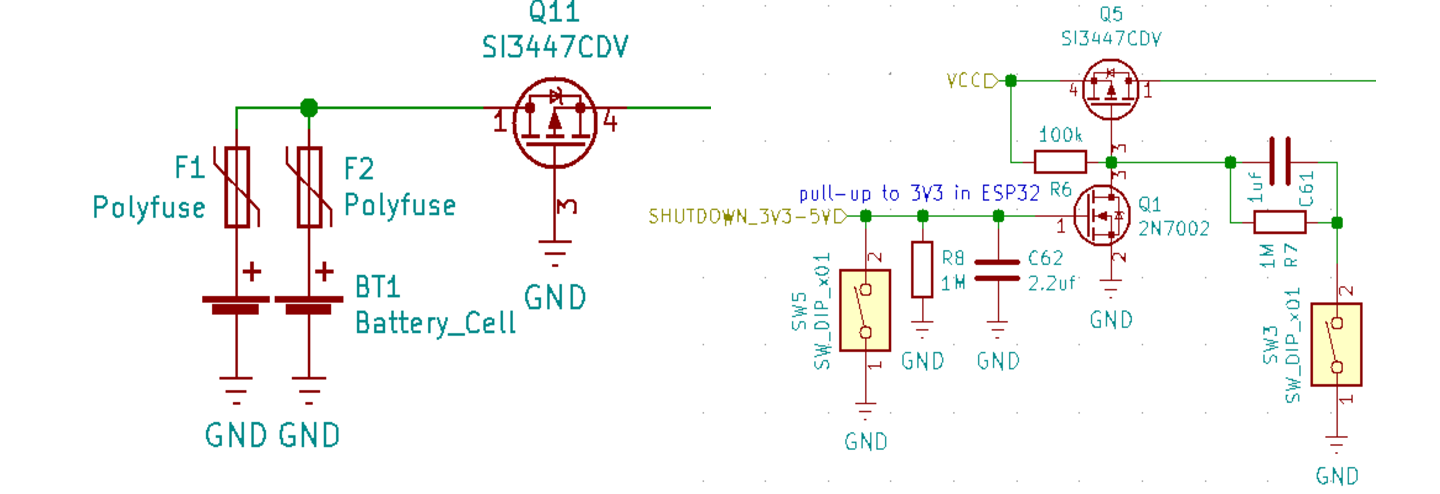
\includegraphics[width=\textwidth]{kapitoly/obrazky/E4/napajeni/ochrana_proti_prepolovani_a_zapinani.png}
    \caption{Ochrana proti přepólovaní a zapínání}
    \label{fig:E4-zapinani}
\end{figure}

\newpage

\paragraph*{Stabilizátor}
\addcontentsline{toc}{paragraph}{Stabilizátor}

Stabilizátor \href{https://datasheet.lcsc.com/szlcsc/1808280153_STMicroelectronics-LD39200PU33R_C222192.pdf}{LD39200} \parencite{ld39200} má pin EN, který slouží k~jeho vypínání. 
Pokud je na nem logická 0, je~stabilizátor vypnut a~pokud 1, je zapnut. Vzhledem k~tomu, že v~mém zapojení toto vypínaní nepotřebuji, je pin EN připojen 
přes R10 přímo na napájecí napětí, a~tak je stabilizátor trvale zapnut.
Konkrétně LD39200 jsem vybral kvůli malému pádu napětí, který vyžaduje pro svůj provoz, typicky 120~mV při proudu 1~A. Vzhledem k~tomu, že~na~vstupu 
mám maximálně 4,2~V, tak maximální napěťový pád, který mám k~dispozici je~0,9~V, protože na výstupu požaduji napětí 3,3~V. Navíc musím počítat 
i~s~vybitou baterií, u~které počítám s~napětím 3,5~V. %Rád bych počítal s~napětím ještě nižším, ale v~nabídce JLCPCB jsem nenašel stabilizátor s~nižším pádem napětí a~zároveň dostatečným proudem.

\begin{figure}[htbp]
    \centering
    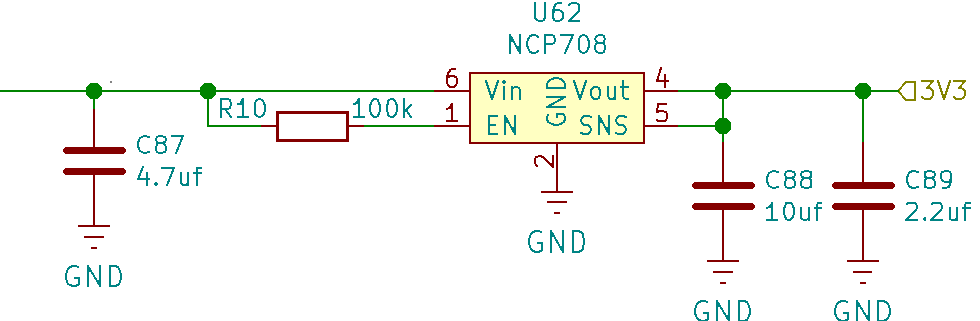
\includegraphics[width=400pt]{kapitoly/obrazky/E4/napajeni/stabilizator.png}
    \caption{Zapojení stabilizátoru}
    \label{fig:E4-stabilizator}
\end{figure}

\paragraph*{Step-up}
\addcontentsline{toc}{paragraph}{Step-up}

\subparagraph*{Step-up vysvětlení funkce}
Zapojení step-upu \footnote{spínaný zdroj který spíná vstupní napětí na napětí vyšší} je~o~něco složitější než stabilizátor, který stačí připojit a funguje. 
Spínané zdroje využívají ke své funkci cívku, na které vzniká změna napětí. Proud cívkou se nedá okamžitě zastavit a právě toho se využívá. 
Když se step-up spustí, připne výstup cívky k~zemi. Ve chvíli, kdy napětí klesně pod zadanou úroveň \footnote{předpokládá se že je v tu chvíli proud cívkou dostatečný}, 
přepne se výstup cívky na výstup step-upu.
Protože proud cívkou se nedá zastavit a~cívkou už proud teče, zvedne se napětí za cívkou, které začne plnit kondenzátor na výstupu.
Když napětí stoupne nad horní hranici požadovaného napětí, výstup cívky se opět přepne na zem. Ve chvíli, kdy napětí na kondenzátorech opět 
klesne, tím že dodává proud, připojí se cívka. Protože se~na~dobu pádu napětí na~výstupním kondenzátoru, připojila cívka na~zem, obnovil 
se~v~ní~proud a~cyklus se tak může opakovat.

\subparagraph*{Step-up zapojení na desce trezoru} 

\footnote{vysvětlení funkce obvodu na obrázku \obr{fig:E4-step-up}}Pro ovládání spínání step-upu jsem zvolil \href{https://datasheet.lcsc.com/szlcsc/Feeling-Tech-FP6276AXR-G1_C83308.pdf}{FP6276}.
Tento obvod jsem zvolil, protože mi vyhovoval jak po stránce napětí tak po~stránce efektivity a~ceny a~zároveň byl v~nabídce firmy JLCPCB
\footnote{firma u~které jsem desky vyráběl a~osazoval}.
Obvod jsem z~většiny zapojil dle doporučení výrobce, mojí prací bylo vlastně jen správně určit hodnoty 
jednotlivých součástek. Na ovládání pinu EN, který FP6276 vypíná, jsem připojil pull-up k napájení a~pro možnost step-up vypnout tranzistor Q2 \parencite{cj3134k}. 
Pokud tedy procesor stáhne dráhu SHUTDOWN 5V k zemi a~tak přivede na G\footnote{GATE, vlastně BASE ale u unipolárního tranzistoru} Q2 zem, 
Q2 se zavře a~tím se na pin EN přivede skrz R18 napájecí napětí, které step-up spustí. 
Pokud se na G Q2 přivede naopak logická jedna, Q2 se~otevře a~na~EN~se~dostane zem, která naopak provoz step-upu zastaví.

\begin{figure}[htbp]
    \centering
    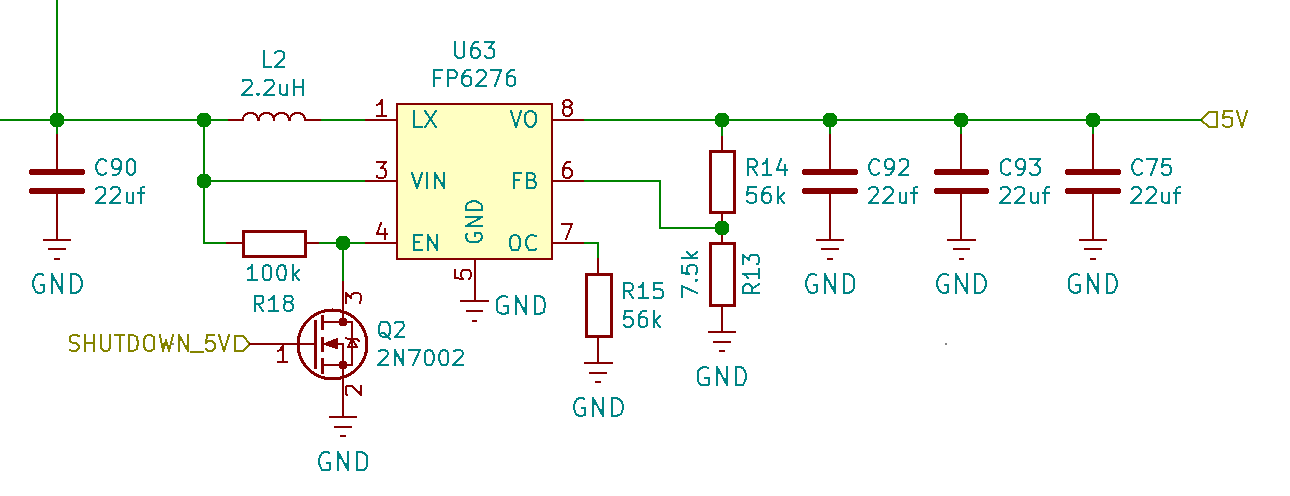
\includegraphics[width=400pt]{kapitoly/obrazky/E4/napajeni/step-up.png}
    \caption{Zapojení step-upu}
    \label{fig:E4-step-up}
\end{figure}

\newpage

\paragraph*{Měření napětí baterií}
\addcontentsline{toc}{paragraph}{měření napětí baterek}

\begin{wrapfigure}{R}{0.4\textwidth}
    \centering
    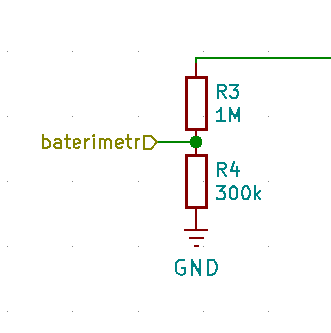
\includegraphics[width=0.4\textwidth]{kapitoly/obrazky/E4/napajeni/delic_baterimetru.png}
    \caption{Měření napětí baterií\label{fig:frog1}}
\end{wrapfigure}

Aby trezor mohl zjistit že má vybité baterie, musí mít možnost jim měřit napětí. ESP32 obsahuje AD převodník takže není problém měřit napětí baterie 
i poměrně přesně, kde však problem nastává, je maximální napětí, které je schopen měřit, a~to 1,1~V. ESP32 sice má možnost připojit k~AD převodníku dělič,
aby se~na~pin dalo přivést napětí až 3,3~V, ale to~pořád není dostatečné, a~také se~tím snižuje přesnost měření. Proto je na desce jednoduchý dělič napětí
složený ze~dvou odporů, jednoho s~hodnotou 1~M$\Omega$ a~druhého 300~k$\Omega$, takže při plně nabitých bateriích bude na výstupu děliče 0,97~V. %todo kolik je tam těch baterek. <- nevim jak to tam teď elegantně dopsat a ani bych to nepovažoval za nějak zvlášť podstatnou informaci v odstavci o měření napětí, je to hned v první větě pod nadpisem napájení

\newpage